% Task recurrence — periodic vs sporadic vs aperiodic release patterns
% Compile:  pdflatex recurrence.tex  &&  dvisvgm --pdf recurrence.pdf
\documentclass[border=4pt]{standalone}
\usepackage{lmodern}
\usepackage{tikz}
\usetikzlibrary{arrows.meta}

\definecolor{kmblue}{HTML}{003874}
\definecolor{kmgold}{HTML}{BA9224}
\definecolor{rtred}{HTML}{E3342F}
\definecolor{dkgray}{HTML}{555555}

\begin{document}
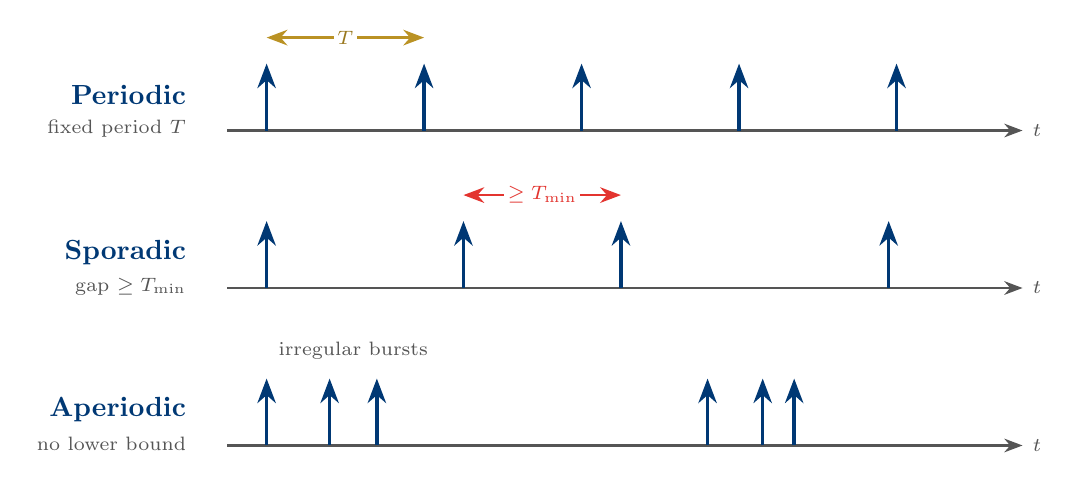
\begin{tikzpicture}[>=Stealth,font=\sffamily,x=1cm,y=1cm]

  % ===== PERIODIC =====
  \node[anchor=east,kmblue,font=\bfseries] at (2.0,5.05) {Periodic};
  \node[anchor=east,dkgray,font=\scriptsize] at (2.0,4.62) {fixed period $T$};
  \draw[->,dkgray,line width=0.8pt] (2.4,4.6) -- (12.5,4.6)
        node[right,font=\scriptsize]{$t$};
  \foreach \x in {2.9,4.9,6.9,8.9,10.9}
    \draw[kmblue,line width=1.3pt,->] (\x,4.6) -- (\x,5.45);
  \draw[<->,kmgold,line width=1.0pt] (2.9,5.78) -- (4.9,5.78);
  \node[kmgold!82!black,font=\scriptsize,fill=white,inner sep=1.2pt]
        at (3.9,5.78) {$T$};

  % ===== SPORADIC =====
  \node[anchor=east,kmblue,font=\bfseries] at (2.0,3.05) {Sporadic};
  \node[anchor=east,dkgray,font=\scriptsize] at (2.0,2.62) {gap $\ge T_{\min}$};
  \draw[->,dkgray,line width=0.8pt] (2.4,2.6) -- (12.5,2.6)
        node[right,font=\scriptsize]{$t$};
  \foreach \x in {2.9,5.4,7.4,10.8}
    \draw[kmblue,line width=1.3pt,->] (\x,2.6) -- (\x,3.45);
  \draw[<->,rtred,line width=1.0pt] (5.4,3.78) -- (7.4,3.78);
  \node[rtred,font=\scriptsize,fill=white,inner sep=1.2pt]
        at (6.4,3.78) {$\ge T_{\min}$};

  % ===== APERIODIC =====
  \node[anchor=east,kmblue,font=\bfseries] at (2.0,1.05) {Aperiodic};
  \node[anchor=east,dkgray,font=\scriptsize] at (2.0,0.62) {no lower bound};
  \draw[->,dkgray,line width=0.8pt] (2.4,0.6) -- (12.5,0.6)
        node[right,font=\scriptsize]{$t$};
  \foreach \x in {2.9,3.7,4.3,8.5,9.2,9.6}
    \draw[kmblue,line width=1.3pt,->] (\x,0.6) -- (\x,1.45);
  \node[dkgray,font=\scriptsize] at (4.0,1.80) {irregular bursts};

\end{tikzpicture}
\end{document}
